\documentclass[12pt,]{article}
\usepackage{lmodern}
\usepackage{amssymb,amsmath}
\usepackage{ifxetex,ifluatex}
\usepackage{fixltx2e} % provides \textsubscript
\ifnum 0\ifxetex 1\fi\ifluatex 1\fi=0 % if pdftex
  \usepackage[T1]{fontenc}
  \usepackage[utf8]{inputenc}
\else % if luatex or xelatex
  \ifxetex
    \usepackage{mathspec}
  \else
    \usepackage{fontspec}
  \fi
  \defaultfontfeatures{Ligatures=TeX,Scale=MatchLowercase}
\fi
% use upquote if available, for straight quotes in verbatim environments
\IfFileExists{upquote.sty}{\usepackage{upquote}}{}
% use microtype if available
\IfFileExists{microtype.sty}{%
\usepackage{microtype}
\UseMicrotypeSet[protrusion]{basicmath} % disable protrusion for tt fonts
}{}
\usepackage[margin=1in]{geometry}
\usepackage{hyperref}
\PassOptionsToPackage{usenames,dvipsnames}{color} % color is loaded by hyperref
\hypersetup{unicode=true,
            pdftitle={Pure Exploration},
            pdfauthor={Tim Radtke},
            colorlinks=true,
            linkcolor=Maroon,
            citecolor=Blue,
            urlcolor=blue,
            breaklinks=true}
\urlstyle{same}  % don't use monospace font for urls
\usepackage{graphicx,grffile}
\makeatletter
\def\maxwidth{\ifdim\Gin@nat@width>\linewidth\linewidth\else\Gin@nat@width\fi}
\def\maxheight{\ifdim\Gin@nat@height>\textheight\textheight\else\Gin@nat@height\fi}
\makeatother
% Scale images if necessary, so that they will not overflow the page
% margins by default, and it is still possible to overwrite the defaults
% using explicit options in \includegraphics[width, height, ...]{}
\setkeys{Gin}{width=\maxwidth,height=\maxheight,keepaspectratio}
\IfFileExists{parskip.sty}{%
\usepackage{parskip}
}{% else
\setlength{\parindent}{0pt}
\setlength{\parskip}{6pt plus 2pt minus 1pt}
}
\setlength{\emergencystretch}{3em}  % prevent overfull lines
\providecommand{\tightlist}{%
  \setlength{\itemsep}{0pt}\setlength{\parskip}{0pt}}
\setcounter{secnumdepth}{5}
% Redefines (sub)paragraphs to behave more like sections
\ifx\paragraph\undefined\else
\let\oldparagraph\paragraph
\renewcommand{\paragraph}[1]{\oldparagraph{#1}\mbox{}}
\fi
\ifx\subparagraph\undefined\else
\let\oldsubparagraph\subparagraph
\renewcommand{\subparagraph}[1]{\oldsubparagraph{#1}\mbox{}}
\fi

%%% Use protect on footnotes to avoid problems with footnotes in titles
\let\rmarkdownfootnote\footnote%
\def\footnote{\protect\rmarkdownfootnote}

%%% Change title format to be more compact
\usepackage{titling}

% Create subtitle command for use in maketitle
\newcommand{\subtitle}[1]{
  \posttitle{
    \begin{center}\large#1\end{center}
    }
}

\setlength{\droptitle}{-2em}
  \title{Pure Exploration}
  \pretitle{\vspace{\droptitle}\centering\huge}
  \posttitle{\par}
  \author{Tim Radtke}
  \preauthor{\centering\large\emph}
  \postauthor{\par}
  \predate{\centering\large\emph}
  \postdate{\par}
  \date{5/3/2017}

\usepackage[retainorgcmds]{IEEEtrantools}
\usepackage{bm}
\usepackage{amsmath}
\newtheorem{theorem}{Theorem}

\begin{document}
\maketitle

In some previous chapter, we must have introduced the Canonical
Exponential Family (see Garivier and Kaufmann, page 3) and the Kullback
Leibler distance; especially also the KL for exponential family, for
Bernoulli and Gaussian in particular, and so that \(kl()\) is defined.

Before this chapter, a general introduction to A/B tests, with general
sampling bounds for two variants case and uniform sampling. Get people
hooked by general application in website optimization?

\subsection{Multi Armed Bandit and Pure
Exploration}\label{multi-armed-bandit-and-pure-exploration}

\label{ch:MABandPureExploration}

We now move beyond the previously described problem of A/B testing by
opening restrictions which we held so far. There are several ways in
which to do that, but the main way will be two no longer require uniform
sampling strategies. Further, we most often are interested in finding
the best among \(K\) arms. Other parts of the literature try to find the
best \(m\) among \(K\) arms.

(What should come first? Paper by Kaufmann et al. about A/B tests but
unifying FC and FB, or first make a differentiation between FB and FC?)

For a start, consider again the idea of sampling \(K\) variants of for
example websites which return a real-valued (as simple as Bernoulli)
feedback coming from distributions \(\nu_k\), \(k \in \{1, \dots, K\}\).
We still want to find the distribution \(k\) for which the mean is equal
to the highest mean among the distributions \(\mu=\mu^*\). To do so, we
are no longer restricted to sampling the distributions in a round-robin
fashion as previously, but we are allowed to set up new sampling
strategies with the general purpose of finding the best arm as quick as
possible with as much confidence as possible.

To be a little more precise, we consider \(K\) probability distributions
\(\nu_1, \dots, \nu_k\) with respective means \(\mu_1, \dots, \mu_k\).
At each round \(t = 1, 2, \dots\), we can decide from which distribution
to sample, that is, we pick an arm
\(A_t \in \mathcal{A} = \{1, \dots, k\}\), and we observe the feedback
\(X_t\) from distribution \(\mu_{A_t}\). What distinguishes this from
the A/B testing setting is the fact that by picking an arm we actively
choose at each time the distribution from which we would like to receive
the next sample. We are no longer restricted to the uniform sampling
strategy. In fact, our goal is define the a sampling strategy
\((A_t)_t\) with characteristics that are to be analyzed and ideally
optimal in a sense to be specified.

In any case, the literature considered in this chapter is concerned with
strategies whose objective it is to identify the best arm defined by
\(\mu^* = \max_{1\leq a \leq K} \mu_a\). In contrast to multi-armed
bandit problems concerned with optimizing regret (Auer et al, Agrawal et
al), such algorithm could in an extreme case sample the best arm only
once but the inferior arms multiple times, if this helps identifying it
as the clearly best arm for some reason. In general, it is only
important to make a single correct decision \emph{after} the final
sample has been drawn.

As described in Garivier and Kaufmann (2016), a general strategy to find
\(\mu^*\) can be defined by three attributes:

(Add sigma field definition???)

\begin{itemize}
\tightlist
\item
  a \emph{sampling rule} \((A_t)_t\)
\item
  a \emph{stopping rule} \(\tau\)
\item
  a \emph{decision rule} \(\hat{a}_t \quad (=\hat{a}_t(\delta))\)
\end{itemize}

This allows to describe the goal then as finding
\(\hat{a}_t \in \arg \max_a \mu_a\) with the largest confidence
\(\delta\) possible while constrained to minimizing the rounds \(\tau\)
needed to find the estimate and confidence.

Recent literature has dealt with this problem by specifying one of
\(\{\tau, \delta\}\) upfront and then optimizing the other. These two
settings are called \emph{fixed budget} (FB) and \emph{fixed confidence}
(FC).

Fixed confidence can seem like a more natural approach to the problems
at first. Especially when considering the notion of statistical
significance and the famous \(\alpha = 0.05\) confidence level that
comes with the attitude of ``We do not accept any difference as
significant unless a difference as large or larger as the one observed
has a probability of less than 5\% assuming there is no effect''. In the
problem of identifying a superior arm, assuming there exists a superior
arm, this notion might lead to very large sample sizes depending on the
effect size. In particular, in the application of web optimization,
where websites are optimized by conversion rate, which might be at a
level of \(0.06\), for example, it would take \(41575\) samples to
detect a 10\% (or larger) difference in conversion rate at a 5\%
significance (and 95\% power)
\href{http://www.evanmiller.org/ab-testing/sample-size.html\#!6;95;5;10;1}{source}.

But in the situation described above, we're not really fixing the
confidence level. We are fixing the number of samples to make sure that
a given effect size could be detected as significant difference at some
confidence level (here, 5\%). But even if the actual difference between
the two versions is less than the minimum detectable effect size, the
test could give us some detected difference at some confidence. Looking
at it this way, the fixed budget setting may actually be more alike to
standard A/B testing procedures, in which a sample size is fixed
\emph{before} the test is run and determined by the minimum detectable
effect, and confidence level and power of the test.

Consequently, the fixed confidence setting is concerned with fixing a
maximal level of risk \(\delta\) that one is willing to accept. While
minimizing the expected sample size called \emph{sample complexity}, a
corresponding strategy needs to fulfill
\(\mathbb{P}(\hat{a}_\tau \notin \arg \max \mu_a)\leq \delta\) (and then
is called \(\delta\)-PAC). Compare Garivier and Kaufmann (2016).

On the other hand, the fixed budget setting describes strategies which
fix the number of samples \(\tau\) upfront and then try to minimize the
probability of error \(\mathbb{P}(\hat{a}_\tau \notin \arg \max \mu_a)\)
of the decision that's made after the last sample has been drawn.

Alternative formulations which are more rare in the literature are so
called \emph{anytime} strategies aiming to optimize the probability of
error and the sample complexity in a way such that the procedure can be
stopped at anytime (after every round) and return a decision with a
certain guaranteed level of risk. See
\href{http://proceedings.mlr.press/v48/jun16-supp.pdf}{Jun and Nowak
(2016)} for one discussion of the topic. The advantage over the fixed
budget case is that users do not have to specify a budget in advance.
This is especially helpful, if it is not foreseeable how many samples
will be available. Since some fixed budget strategies explore arms in
stages, they might not be able to guarantee a confidence when stopped
before their budgeted rounds.

Other literature tries to analyze the two settings of fixed budget and
fixed confidence seperately, but to make them comparable by using
complexity measures for problems that are on the same scale (see
Kaufmann et al. 2016, Kaufmann et al. 2017). We will come back to this
topic in chapter \ldots{}

\subsubsection{Fixed Confidence}\label{fixed-confidence}

The setting of fixed confidence can be framed as a sequential testing
problem. After each round, we might ask ourselves whether we have
sufficient evidence to make a \(\delta\)-PAC decision. If we cannot make
such decision, we continue to draw the next sample. And because we are
not restricted to uniform sampling strategies, we pull the next sample
so as to gain as much information with the purpose of minimizing the
expected overall number of samples until we can make the \(\delta\)-PAC
decision.

Descriptions like this lead back to Chernoff (1959) describing settings
in which experiments (arms) are performed sequentially. After each
round, it has to be decided whether a next experiment is performed or
whether the final decision is made based on a hypothesis test where the
decision selects between one of two actions. In contrast to the modern
literature, Chernoff takes into account the cost that samples have and
acknowledges that his derivations hold when the cost of sampling goes to
zero. In particular, he compares two Bernoulli distributions based on
their means \(\mu_1, \mu_2\). The problem is formulated as hypotheses,
with \(H_0: \mu_1 > \mu_2\) and \(H_1: \mu_1 \leq \mu_2\). After \(n\)
samples, one observes for the paramater vector \(\mu = (\mu_1, \mu_2)\)
the maximum likelihood estimate
\(\hat{\mu} = (\hat{\mu}_1, \hat{\mu}_2)=(m_1/n_1, m_2/n_2)\), where
\(m_1\) are the successes from distribution 1 after \(n_1\) pulls.
Assuming \(\hat{\mu}_1 > \hat{\mu}_2\), and assuming that we believe
this is the actual state of the world, \(\mu =\hat{\mu}\), we assume
\(H_0\) and want to test it against the alternative \(H_1\) represented
by \(\stackrel{\sim}{\mu}\), which is an undefined vector with some
\(\stackrel{\sim}{\mu}_1 \leq \stackrel{\sim}{\mu}_2\) so that \(H_1\)
holds.

Coming from sequential likelihood-ratio tests, Chernoff motivates the
use of the Kullback-Leibler divergence to determine from which
distribution to sample next. He computes the divergence for the first
distribution comparing \(\hat{\mu}_1\) and \(\stackrel{\sim}{\mu}_1\),
as well as the divergence for the second distribution comparing
\(\hat{\mu}_2\) with \(\stackrel{\sim}{\mu}_2\). Chernoff shows to pick
the distribution next which maximizes the Kullback-Leibler divergence.
The intuition for this comes from how Chernoff computes the alternative
\(\stackrel{\sim}{\mu}\). It holds that \(\stackrel{\sim}{\mu}_1\) =
\(\stackrel{\sim}{\mu}_2\) = \(\stackrel{\sim}{\mu}_i\), where
\(\stackrel{\sim}{\mu}_i\) is a weighted average of \(\hat{\mu}_1\) and
\(\hat{\mu}_2\). As noted by Chernoff (page 759), the weights
\((1-\lambda, \lambda)\) are proportional to how often each distribution
has been sampled.

Now, what happens is that long term, we expect the maximum likelihood
estimates \(\hat{\mu}\) to be close to \(\mu\). At the same time, given
that \(\hat{\mu}\) does not fluctuate much anymore, there will be
weights \((1-\lambda, \lambda)\) such that the two distributions are
sampled in fixed proportions (a share of \(\lambda\) for the second
distribution), and the Kullback-Leibler divergence for each distribution
will be equal:
\(D_{KL}(\mu_1, \stackrel{\sim}{\mu}_i^*, \nu_1) = D_{KL}(\mu_2, \stackrel{\sim}{\mu}_i^*, \nu_2)\),
where \(\stackrel{\sim}{\mu}_i^* = (1-\lambda) \mu_1 + \lambda \mu_2\).

(Is this not just the Chernoff Information as described in Garivier \&
Kaufmann page 6?)

This observation can be interpreted similar to how under standard
composite hypothesis testing, one compares the \(H_1\) against the value
under \(H_0\) that is the closest to \(H_1\). For example, if we observe
samples from a normal distribution and estimate the mean with the sample
mean which is observed to be positive, \(\hat{\mu}>0\), we might want to
test \(H_0: \mu \leq 0\) against \(H_1: \mu > 0\). To do so, we compare
\(\hat{\mu}\) against the value \(\mu_{H_0} \in (\infty, 0]\) closest to
\(H_1\); thus \(\mu_{H_0} = 0\).

In our case, as argued by Chernoff, the mean vector closest to \(\mu\)
under the alternative hypothesis is given by \(\stackrel{\sim}{\mu}^*\).
Under this value, it is the most difficult to properly distinguish
between the different hypotheses. It is the point at which we stand the
worst chances to gain new information from sampling any of the two arms
(as represented by the fact that both Kullback-Leibler divergences are
equal). Consequently (ELABORATE!?),
\(\stackrel{\sim}{\mu}^* = \arg \min_{\stackrel{\sim}{\mu}} \max_{\nu_i} D_{KL}(\mu, \stackrel{\sim}{\mu}, \nu_i)\).

This result can be described as the solution to a zero-sum two-player
minimax game, in which

\begin{itemize}
\tightlist
\item
  the experimenter picks from which distribution to sample from with the
  goal of maximizing \(D_{KL}\)
\item
  then the opponent picks the alternative specification true under the
  alternative hypothesis to minimize \(D_{KL}\)
\end{itemize}

and the value of the game is given by
\(\max_{\nu} \min_{\omega} D_{KL}(\mu, \omega, \nu)\). Then, with the
opponent picking \(\omega = \stackrel{\sim}{\mu}^*\), the experimenter
will choose the randomized maxmin strategy of picking \(\nu_1\) and
\(\nu_2\) in proportions \((1-\lambda)\) and \(\lambda\).

Very similar games have been described by by Russo (2016) and Garivier
and Kaufmann (2016). Both analyze settings of pure exploration bandits
with fixed confidence. While Garivier and Kaufmann find the game as part
of their lower bound on the sample complexity
\(\mathbb{E}_{\mu}[\tau_{\delta}]\) in their theorem 1, Russo finds his
version when deriving the posterior probability on selecting the wrong
arm and determines that the solution to the game describes the
asymptotically optimal allocation of draws for each arm (page 17).

However, as pointed out by Russo (2016), this game is based on the
knowledge of the true parameter \(\mu\) (\(\bm{\theta}^*\) in his
notation) and thus the optimal allocation is not readily available when
designing an algorithm to solve the exploration problem. Instead, he
shows that his algorithms reach the optimal allocation asymptotically
eventhough they do not actively try to solve maxmin game.

(Put in more exact description of the problem solved by Russo so that
one can exactly compare the different games and the exponents given by
Russo and Garivier \& Kaufmann)

In contrast, Garivier and Kaufmann (2016) do devise a sampling rule that
is based on estimating the optimal sampling proportions
\(w^*(\bm{\mu})\) based on the current estimates \(\hat{\mu}(t)\)
leading to the plug-in estimates \(w^*(\hat{\mu}(t))\). However, the
authors acknowledge the fact that using these plug-in estimates in order
to estimate the optimal sampling proportions may well lead to problems
if the initial estimates \(\hat{\mu}(t)\) are off for small \(t\). A bad
estimate can lead the bandit algorithm to abandon an arm in the further
sampling. Then, an arm that should be explored more -- which would lead
to a fix of the initial estimate -- might not be explored and distort
the overall proportions and in the worst case the final decision. In the
description of Garivier and Kaufmann, such sampling rule based on
plug-in estimates would simply fail from time to time. Thus, they adjust
the solution of the optimization problem solving for \(w^*\) in order to
enforce sufficient exploration of arms, see their lemma 7. More
straightforward however is the adjustment in their \emph{D-Tracking}
rule in lemma 8, which checks every round whether there exists any arm
with pulls \(N_a(t) < \sqrt{t} - K/2\) lacking behind the other arms. If
this is fulfilled, the arm with the least amount of pulls is pulled.
Else, the pull is determined by the plug-in estimates. These rules then
also satisfy what was described by Russo: Their empirical sampling
proportions converge to the optimal proportions, compare proposition 9
in Garivier and Kaufmann (2016) and proposition 7 in Russo (2016).

\paragraph{Game, and Lower Bound on the Sample
Complexity}\label{game-and-lower-bound-on-the-sample-complexity}

We will now derive the lower bound on the sample complexity in the fixed
confidence bandit setting demonstrated in Garivier and Kaufmann (2016).

Consider again the setting as defined in section
\ref{ch:MABandPureExploration}. For their lower bound, Garivier and
Kaufmann (2016) consider bandit models where the distributions come from
one-parameter exponential families. Consequently, the distributions can
be parameterized by their means. Therefore, if we let \(\mathcal{S}\) to
be a set of bandit models with \(K\) distributions each, then each model
is fully defined by a vector \(\bm{\mu} = (\mu_1, \dots, \mu_K)\).
Assume that every \(\bm{\mu} \in \mathcal{S}\) has a unique maximum
given by \(a^*(\bm{\mu})\) such that
\(\mu_{a^*} > \max_{a \neq a^*(\bm{\mu})} \mu_a\). In order to fix the
confidence, we specify the risk \(\delta\). The strategies corresponding
to this risk are called \(\delta\)-PAC if for every
\(\bm{\mu} \in \mathcal{S}\),
\(\mathbb{P}_{\bm{\mu}}(\tau_{\delta} < \infty) = 1\) (the strategy ends
surely with after finite samples) and
\(\mathbb{P}_{\bm{\mu}}(\hat{a}_{\tau_{\delta}} \neq a^*) \leq \delta\)
(the probability of picking not the optimal arm is smaller than the
fixed risk). As in Garivier and Kaufmann, we introduce the set of
problems for which the optimal arm is different from the one in
\(\bm{\mu}\):

\begin{equation*}
\text{Alt}(\bm{\mu}) := \{\bm{\lambda} \in \mathcal{S}: a^*(\bm{\lambda}) \neq a^*(\bm{\mu})\}
\end{equation*}

where \(\bm{\lambda}\) is the vector of means defining the distributions
of the alternative problem to \(\bm{\mu}\). Lastly, we have the set of
probability distributions on the arms \(\mathcal{A}\):
\(\Sigma_K = \{w \in \mathbb{R}_{+}^K: w_1 + \dots + w_K = 1\}\).
\marginpar{Give more intuition for what these probability distributions are}
We are now ready to state the theorem.

\begin{theorem}[Garivier and Kaufmann, 2016] \label{theorem:GarivierKaufmannTheorem1}
Let $\delta \in (0,1)$. For any $\delta$-PAC strategy and any bandit model $\bm{\mu} \in \mathcal{S}$,

\begin{equation*}
\mathbb{E}_{\bm{\mu}} [\tau_{\delta}] \geq T^*(\bm{\mu}) \text{\em{kl}}(\delta,1-\delta),
\end{equation*}

where 

\begin{equation} \label{eq:GarivierKaufmann_Theorem1_Game}
T^*(\bm{\mu})^{-1} := \sup_{w \in \Sigma_K} \inf_{\bm{\lambda} \in \text{\em{Alt}}(\bm{\mu})} \left( \sum_{a=1}^K w_a d(\mu_a, \lambda_a)\right) .
\end{equation}
\end{theorem}

In equation \eqref{eq:GarivierKaufmann_Theorem1_Game}, we again see the
game occur that we describe above. In this case, the game is about the
minimal number of rounds \(T = T(w,\lambda)\) needed for any bandit
strategy to ensure that the strategy fulfills the \(\delta\)-PAC
constraint. Consider that we have the inverse of \(T\) in equation
\eqref{eq:GarivierKaufmann_Theorem1_Game}. Then we see that

\begin{itemize}
\tightlist
\item
  the statistician tries to minimize the number of rounds by choosing
  the optimal proportions of draws \(w^*\) for each arm
\item
  the opponent picks the alternative model \(\bm{\lambda}\) so as to
  maximize the number of necessary rounds
\end{itemize}

When choosing \(\bm{\lambda}\), the opponent will choose an alternative
as close to the original model as possible so as to minimize the
Kullback-Leibler divergence \(d(\mu_a, \lambda_a)\). As already noted in
Chernoff (1959), this will minimize the information available to the
statistician and make it difficult to distinguish between the cases with
confidence.

\begin{figure}[htbp]
\centering
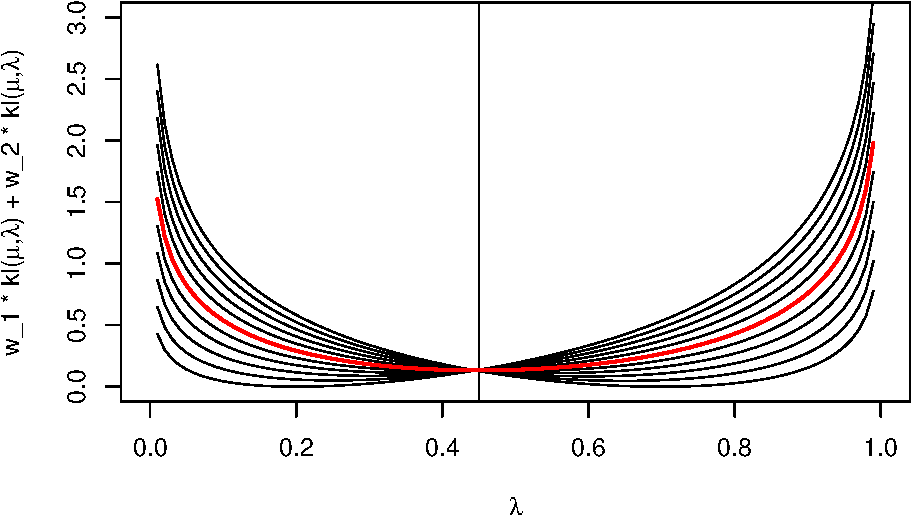
\includegraphics{Pure_Exploration_files/figure-latex/unnamed-chunk-1-1.pdf}
\caption{Statistician chooses the curve by picking the weights w, then
the opponent picks lambda. In the case of a two-armed bandit, we have
w1+w2 = 1. The plot suggests that uniform allocation is optimal for
Bernoulli bandits. The thick line shows the result for w1=w2=0.5.}
\end{figure}

The plot above specifies again the game and the reasoning of the
opponent. Given a model \(\bm{\mu} = (\mu_1, \dots, \mu_K)\) with
\(\mu_1 > \mu_2 \geq \dots \geq \mu_K\), the experimenter chooses the
proportions of arm draws \(w = (w_a)_a\). Then the opponent chooses an
arm \(a \in \{2, \dots, K\}\) and chooses the alternative distribution
for arm \(a\),
\(\lambda_a = \arg \min_{\lambda} w_1 d(\mu_1, \lambda) + w_a d(\mu_a, \lambda)\).
The payoff of the game is then the minimal number of rounds \(T\) so
that the restriction
\(Tw_1 d(\mu_1, \lambda_a - \epsilon) + Tw_a d(\mu_a, \lambda + \epsilon) \geq \text{kl}(\delta, 1-\delta)\)
holds when \(a^*(\bm{\mu}) \neq a^*(\bm{\lambda})\) due to \(\epsilon\).
Consequently, the value is given by

\begin{equation}
T(w, a, \delta) = \frac{\text{kl}(\delta, 1-\delta)}{w_1 d(\mu_1, \lambda_a - \epsilon) + w_a d(\mu_a, \lambda + \epsilon)}
\end{equation}

which is comparable to the result in Theorem (Garivier and Kaufmann,
2016) \ref{theorem:GarivierKaufmannTheorem1}.

\subsubsection{Fixed Budget}\label{fixed-budget}

Given the success of UCB, why not try it for this problem as well?

-\textgreater{} What would be the equivalent algorithm? -\textgreater{}
Audibert et al. (2009) -\textgreater{} Adjustment proposed by Audibert
et al. (2015) -\textgreater{} Choose a linear in t to explore more!
-\textgreater{} Show upper bound -\textgreater{} Give at least the
standard steps of lower bound proof


\end{document}
